\chapter{基本物理}

\section{引言}

在本章中,我们将考察有关物理学的最基本概念——即我们在目前所知道的事物的本性。这里将不去涉及我们如何知道所有这些观念是正确的那个认识过程,你们在适当的时候会学习到这些具体的细节。

我们在科学上所关心的事物,具有无数形式和许多属性。举例来说,假如我们站在岸边眺望大海,将会看到:这里有海水、拍击的浪花、飞溅的泡沫以及汹涌的波浪,还有太阳、光线、蔚蓝的天空、白云以及空气的流动——风;在海边有沙粒,不同色纹和硬度的岩石;在海里浮游着生物,此生彼灭;最后,还有我们这些站在海岸边的观察者;甚至还有幸福和怀念。在自然界的其他场合,难道不也同样出现如此纷繁复杂的事物和影响吗?无论在哪里,到处都是这样错综复杂和变化无穷。好奇心驱使我们提出问题,把事物联系起来,而将它们的种种表现理解为:或许是由较少量的基本事物和相互作用以无穷多的方式组合后所产生的结果。

例如,沙粒和岩石是两回事吗?就是说,沙粒只不过是大量的细小石块吗?月亮是不是一块巨大的岩石呢?如果我们了解岩石,是否就能了解沙粒和月亮呢?风是否与海洋中的水流相似,就是一种空气的流动?不同的运动有什么共同特征?不同的声音有什么相似之处?究竟有多少种颜色?等等,等等。我们就是试图这样地逐步分析所有的事情,把那些乍看起来似乎不相同的东西联系起来,希望有可能\uwave{减少不同类}事物的数目,从而能更好的理解它们。

几个世纪以前,人们想出了一种部分解答这类问题的方法,那就是:\uwave{观察},\uwave{推理}和\uwave{实验};这些内容构成了通常所说的\uwave{科学方法}。在这里,我们将只限于对那些有时称之为基本物理中的基本观点,或者由于应用科学方法而形成的基本概念作一描述。

现在我们要问:所谓“理解”某种事情指的是什么意思?可以作一想象:组成这个“世界”的运动物体的复杂排列似乎有点像是天神们所下的一盘伟大的象棋(这里指的是国际象棋——译者注),我们则是这盘棋的观众。我们不知道弈棋的规则,所有能做的事情就是\uwave{观看}这场棋赛。当然,假如我们观看了足够长的时间,总归能看出几条规则来,这些弈棋规则就是我们所说的基本物理。但是,即使我们知道了每条规则,仍然有可能不理解为什么下棋时要走某一步棋,这仅仅是因为情况太复杂了,而我们的智力却是有限的。如果你们会下棋,就一定知道,学会所有的规则是容易的,但是,要选择最好的一着棋,或者要弄懂别人为什么走这一着棋,往往就很困难了。在自然界里,也正是如此,而且只有更难一些。但是,至少我们能发现所有的规则。实际上我们今天还没找到一切规则(时而会出现一些像弈棋中“以车护王”那样的情况,使我们仍然感到无法理解)。除此之外,我们确实能用已知规则来解释的事情也是非常有限的,因为几乎所有的情况都是极其复杂的,我们不能领会这盘棋中应用这些规则的走法,更无法预言下一步将要怎样。所以,我们必须使自己只限于弈棋规则这个比较基本的问题。如果我们知道了规则,就认为“理解”了世界。

如果我们不能很好的分析这盘象棋游戏,那么又怎样来辨别我们“猜测”出的规则实际上是否正确呢?大致地讲,可以有三种办法。第一,可能有这种情况:大自然安排的,或者说我们将大自然安排的十分简单,只有少数几个组成部分,从而使我们能够正确地预测将要发生的事。在这种情况下,就能检验我们的规则是怎样起作用的。(在棋盘角落里可能只有少数几个棋子在移动,所以我们能够正确地解决。)

第二种检验规则的好办法是,利用那些由已知规则推导出来的一些较一般性的法则来检验已知规则本身。比如,象在棋盘中移动的规则是只许走对角线,因而我们可以推断,无论象走了多少步,它总是出现在红方块里。这样,即使不能领会细节,我们也总能检验有关象的走法的概念,只要弄清楚它是否一直在红方块里。当然,在相当长的时间里,它都将如此,直到突然发现它出现在黑方块里。(显然,这时发生的情况是这个象被俘获了,另一个卒走过来成为皇后,红方块里的象就变成黑方块里的象。)这也就是物理学中出现的情况,即使我们不能领会其中的细节,但是在相当长的时期内我们仍有在各方面都很好地起作用的规则;但是在某个时候,我们又会发现新的规则。从基本物理的观点来看,最有趣的现象当然是在那些\uwave{新的}场合——那些已知规则行不通的场合中所出现的现象,而不是在原有规则行得通的地方发生的现象!这是我们发现新规则的一条途径。

第三个鉴别我们的观念是否正确的方法比较粗糙,但或许是所有方法中最为有效的。这就是用粗略的近似方法来加以辨别。我们可能说不出为什么阿莱克因(Alekhine)\footnote{世界著名弈棋手,系国际象棋大师。曾多次获得国际象棋世界冠军。——译者注}要走这步棋,但是我们或许能大致认为它或多或少地在调集一些棋子到王的周围来保护它。因为这是在这种情况下明摆着的事。同样,根据我们对这盘棋的理解,即使不能看出每一步棋的作用,也常常能对自然界多少有所理解。

人们首先把自然界中的现象大致分为几类,如热、电、力学、磁、物性、化学、光或光学、X射线、核物理、引力、介子等等现象。然而,这样做的目的,是将\uwave{整个自然界}看作是一系列现象的许多不同侧面。这就是今天基础理论物理面临的问题:\uwave{发现隐匿在实验后的定律};\uwave{把各类现象综合起来}。在历史上,人们总能做到这一点,但随着时间的推移,新的事实发现了;我们曾经将现象综合得很好,突然,发现了 X 射线,随后我们又融合了更多事实,但是又发现了介子。因此,在弈棋的任何一个阶段,看起来总是相当凌乱。大量事实被归并了,但总还有许多线索向一切方向延伸出去。这就是今天的状况,也就是我们将试图去描绘的现状。

历史上出现过的若干进行综合的情况有如下几个。首先,是\uwave{热}与\uwave{力学}的综合,当原子运动时,运动得越是剧烈,系统所包含的热量就越多,这样,\uwave{热和所有的温度效应}可以用力学定律来说明。另一个巨大的综合,是发现了电、磁、光之间的联系,从而知道它们是同一件事物的不同方面,即今天我们称为\uwave{电磁场}的那个东西的不同表现。还有一个综合,是把化学现象、各种物质的各种性质以及原子的行为统一起来,这就是\uwave{量子化学}的内容。

显然,现在的问题是:能不能继续把所有的事情都综合起来,并且仅仅发现这整个世界体现了\uwave{一件}事情的种种不同方面?无人知道答案如何,我们所知道的只是:这样做下去时,我们发现可以综合一些事实,随后又发觉出现了一些不能综合的事实。我们继续尝试这种拼图游戏。至于是否只有有限数量的棋子,甚至这场拼图游戏是否有底,当然不知道。除非有那么一天终于把拼图拼成了,否则我们就永远不会知道事情的究竟。在这里我们要做的是,看看那种综合已经到了什么程度,在借助于最少的一组原理来理解基本现象方面,现状又是如何。简言之,\uwave{事物是用什么构成的}?\uwave{总共存在多少基本元素}?

\section{1920年以前的物理学}

一开始就从现在的观点讲起是有点困难的,所以让我们先来看一下在1920年左右人们是怎样看待世界的,然后再从这幅图像中挑出几件事情来。在1920年以前,我们的世界图像大致是这样的:宇宙活动的“舞台”是欧几里德所描绘的三维几何\uwave{空间},一切事物在称为\uwave{时间}的某一种媒质里变化,舞台上的基本元素是\uwave{粒子},例如原子,它们具有某些\uwave{特性},首先一个特性是惯性:如果一个粒子正在运动,那么它将沿着同一个方向继续运动下去,除非有\uwave{力}作用其上。此外,第二个基本元素就是\uwave{力},当时认为共有两类力。第一类力是一种极其复杂细致的相互作用,它们以复杂的方式将各种各样的原子约束在不同的组合之中,它们确定当温度升高时,食盐是溶解的更快还是更慢些;另一类已知的力是一种长程的相互作用,它是与距离平方成反比的变化平缓的作用力,称为万有引力。这条定律已为我们所知,它是很简单的。当然,\uwave{为什么}物体的运动一经开始就能保持下去,或者说\uwave{为什么}存在一条万有引力定律,我们则不清楚。

对自然的描述正是我们在这里要关心的。从这个观点出发,气体以及实际上\uwave{所有}的物质都是无数运动着的原子。这样,我们站在海边所听见到的许多东西马上可以联系起来了。首先是压力,它是来自原子与墙或者某个东西的碰撞;如果原子的运动平均而言都是沿着一个方向,这种原子的漂移运动就是风;而无规则的内部运动就是热。某个地方有过多的原子集结在一起时,就形成了过剩密度的波,当波前进时,把成堆的原子推向更远的地方,等等。这种过剩密度的波就是声波。能够理解这么多事情的确是惊人的成就。在前一章里,我们已经说明过一些这样的事情。

粒子有哪些种类?在当时认为有 92 种:那时已经发现有 92 种不同的原子,各按其化学性质而被赋予不同的名称。

其次的问题是“短程力”是什么?为什么碳吸引一个(有时两个)而不是三个氧?原子间的相互作用的机制是什么?是万有引力吗?答案是否定的。万有引力实在是太弱了。于是让我们来设想一种类似于力与距离平方成反比的力,不过在强度上远远超过前者,此外还有一个差别:在重力作用下,每个物体彼此吸引,但现在我们设想有\uwave{两}类“物体”,而这种新的力(当然就是所谓电力)具有同号相斥而异号相吸的特性。具有这样强的作用的“物体”就称为\uwave{电荷}。

那么,我们会得到什么结果呢?假定我们有两个异号电荷,一正一负,并且彼此十分靠近。现在,在若干距离之外,还有另一个电荷。它会感到吸引吗?\uwave{实际上}它几乎\uwave{不}会感到什么作用,因为如果前两个电荷的大小相等,来自一个电荷的吸引被来自另一个电荷的排斥所抵消。所以,在任何可观的距离外只有很小的一点作用力。另一方面,如果我们使第三个电荷\uwave{非常靠近}前两个时,就会发生吸引作用。因为同号电荷的斥力与异号电荷的引力倾向于使异号电荷靠近而使同号电荷远离。这样,排斥作用就将小于吸引作用。这就是为什么由正、负电荷组成的原子相互离开较远时只能感受到很小一点作用力(重力除外),而当它们彼此靠近时,就能够互相“看到内部”而重新安排其电荷,结果产生了极强的相互作用。原子间作用力的最终基础是电的作用。由于这种力是如此巨大,以至所有正的与负的电荷通常都以尽可能紧密的方式结合在一起。所有的事物,甚至我们自己,都由极精细的和彼此强烈作用着的正、负微粒所组成,所有正的微粒与所有负的微粒正好抵消。有时,碰巧我们“擦”去了一些负电荷或正电荷(通常擦去负电荷较为容易),在这种情况下将会发现电力\uwave{不再平衡},于是就能看到电的吸引作用。

为了对电力作用究竟比引力作用大多少有个概念,我们举出大小为 1 毫米,相距为 30 米的两粒沙子为例。假如它们之间的作用力没有抵消,每个电荷都吸引所有其他电荷而不考虑同号电荷间的斥力,因此不会抵消,那么,两颗沙粒之间的作用力会有多大呢?两者间将会产生三百万吨的力!你瞧,只要正电荷或负电荷的数目有一点点\uwave{极小}的过剩或欠缺,就足以产生可观的电效应。当然,这就是你们为什么不能看出带电体与非带电体之间的差别的原因——所牵涉的粒子数目少得无论在物体的重量上或者形状上都很难造成什么差别。

有了这样的图像,对原子就比较容易理解了。人们认为原子的中心是一个带正电的质量甚大的“原子核”,核周围围绕着一定数量的很轻而且带有负电的“电子”。让我们稍稍超前一点提一下:在原子核里也发现了两类粒子——质子和中子,它们的重量几乎相同,并且十分重。质子带正电,中子则呈中性。如果我们有一个原子,其核内有六个质子,从而四周环绕六个电子(在通常的物质世界中负粒子都是电子,与组成原子核的质子和中子相比,它们是很轻的)。在元素周期表上这个原子的序数是 6,名称是碳。原子序数为 8 的物质叫做氧,等等。因为化学性质取决于核外的电子,实际上它只取决于核外有\uwave{多少}电子。所以,一种物质的\uwave{化学}性质只由电子的数目所决定。(化学家的全部元素的名称实际上可以用 1,2,3,4,5 等等编号来称呼。)我们可以说“元素六”,表示六个电子,以代替“碳”这个名称。当然,在先前发现元素时,人们并不知道它们可以用这种方式来编号。此外,这又会使事情复杂化,因此,宁可对这些元素定一个名称和符号,这比用编号来称呼元素来得更好。

关于电的作用,人们还发现了更多事情。对电相互作用的自然解释是,两个物体简单地互相吸引:正的吸引负的。然而后来发现用这种观点来描写电的相互作用并不妥当。更合适的描述这种情况的观点是:在某种意义上,正电荷的存在使空间的“状况”发生畸变,或者说在空间造成了一种“状况”。于是当我们将负电荷放到这个空间里后,它就会感受到一个作用力。这种产生力的潜在可能性就叫做\uwave{电场}。当把一个电子放入电场时,我们就说它受到“拉拽”。于是我们就有两条规则:(1)电荷产生电场;(2)电荷在电场中会受到力的作用而运动。如果我们讨论下述现象的话,建立这条规则的理由就清楚了:假如我们使某物体比方说梳子带电,然后把一张带电的纸片放在一定距离之外,当我们来回移动梳子时,纸片就会有反应,并且总是指向梳子。如果我们使梳子晃动的快些,就会发现纸片的运动有一点滞后,即作用有所延迟。(起先,当我们相当慢地晃动梳子时,我们发现一种错综复杂的现象,这就是磁。磁的影响与作相对运动的电荷有关,所以磁力和电的作用力实际上可以归之于一个场,这象同一件事的两个不同的方面。变化的电场不能离开磁而存在!)假如我们把纸片移得更远,滞后就更大。这时能观察到一件有趣的事:虽然两个带电体之间的作用力应当与距离的\uwave{平方}成反比,但是我们发现当摇动一个电荷时,电作用的影响范围要比起初所猜想的\uwave{大得多}。这就是说,作用的减弱要比反平方的规则来的慢。

这里有一个类比:如果我们在水池里,而在近处漂浮着一个软木塞,我们可以用另一个软木塞划水来“直接”移动那个木塞。如果现在你只注意两个\uwave{软木塞},你能看到的将是一个立即响应另一个的运动——在软木塞之间存在着某种“相互作用”。当然,我们实际上所做的只是搅动了\uwave{水};然后水又去扰动另一个木塞。于是,我们就能提出一条“定律”:如果稍微划一下水,那么水中附近的物体就会移动。当然,假若第二个软木塞离得较远,它将几乎不动,因为我们只是\uwave{局部地}搅动水。另一方面,假如我们晃动木塞,就会产生一个新的现象,这部分水推动了那部分水,等等,于是\uwave{波}就传播开去。这样,由于晃动,就有一种波及\uwave{十分远}的影响和一种振荡的影响,这是无法用直接相互作用来理解的。所以那种直接作用的概念必须用水的存在来代替,或者,对于电的情形,用我们所谓的电磁场来代替。

电磁场能传送各种波。其中的一些就是\uwave{光}波,另一些波用在\uwave{无线电广播里}。但它们总的名称是\uwave{电磁波}。这些振荡的波可以有各种\uwave{频率},一种波和另一种波之间的唯一的真正差别只是\uwave{振荡的频率}。假如我们越来越快地来回晃动电荷,并且注视着所产生的效应时,我们将得到一系列不同的效应,只要用一个数,即每秒钟振荡的次数,就能把这些效应统一起来。通常在我们住房墙上电路里流动电流所产生的扰动约为 100 周/秒。如果我们把频率提高到每秒 500 千周或 1000 千周(1 千周 = 1000 周),我们就“在空气中”了\footnote{原文为“On the air”,直译为“在空气中”,亦作电台“正在广播”解。作者在这里用的是双关语,故有下文的“广播与空气毫无关系”。——译者注}因为这正是无线电广播所用的频率范围(当然,广播与\uwave{空气}毫无关系!没有任何空气也能进行广播)。假如再提高频率,那么就进入调频广播和电视所用的波段。再上去,我们使用一种极短的波,比如雷达所用的波。频率再增高,我们就无需用仪器来“看”这种波了,而用眼睛就能看到它。在频率范围为每秒$ 5\times10^{14} $  到$ 5\times10^{15}  $ 周的时候,只要有可能使带电的梳子晃动的这样快,我们的眼睛就能见到带电梳子的振动像红光、蓝光或紫光,视振动的频率而定。低于上述频率范围的称为红外,高于此范围的称紫外。从物理学家的观点来看,我们能看见某种频率范围的波这个事实并不使这一部分电磁波谱比其他部分有什么更令人注意的地方,但是从人类的观点来看,这当然\uwave{是}更有趣的。如果我们把频率提得更高,于是就得到 X 射线,X 射线不是别的,只是频率极高的光而已。如果再提高频率,就得到 γ 射线。X 射线与 γ 射线这两个名称在使用时几乎是同义的,通常将原子核发出的电磁射线称为 γ 射线,而从原子中发出的这种高能的电磁射线就成为 X 射线,但是不论它们的起源如何,当频率相同时,它们在物理上是无法区别的。如果我们能进到更高的频率,比如说每秒$10^{24}$周,我们发现可以人工制造这样的波,例如用加里福尼亚工学院的同步加速器。我们还可以在宇宙射线里发现频率出奇地高——具有甚至快1000倍的振荡——的电磁波,而这些波目前还不能由我们来控制。

\begin{table}[H]
    \centering
    \label{tab:电磁波谱}
    \caption{电磁波谱}
    \medskip 
    \begin{tabular}{@{}lll@{}}
        \toprule
        频率(周/秒)                     & 名称         & 大略行为 \\ \midrule
        $10^{2}$                    & 电扰动        & 场    \\
        $5\times10^{5}\sim10^{6}$   & 无线电广播      & 波    \\
        $10^{8}$                    & FM-TV      & 波    \\
        $10^{10}$                   & 雷达         & 波    \\
        $5\times10^{14}\sim10^{15}$ & 光          & 波    \\
        $10^{18}$                   & X射线        & 粒子   \\
        $10^{21}$                   & γ射线(核)     & 粒子   \\
        $10^{24}$                   & γ射线(“人造”)  & 粒子   \\
        $10^{27}$                   & γ射线(宇宙射线中) & 粒子  \\ \bottomrule
    \end{tabular}
\end{table}


\section{量子物理学}

说明了电磁场概念和电磁场能传送波后,我们很快就认识到,这些波的行为实际上十分奇怪,看起来完全不像波。在频率较高时,它们的行为更像\uwave{粒子}!正是在1920年后发展起来的量子力学解释了这种奇怪的行为。在1920年之前,爱因斯坦已改变了把空间看作是三维空间、把时间看成是单独存在的这种图像。他首先把它们组合在一起,并称之为空-时,然后又进一步用弯曲的空-时来描绘万有引力。这样,宇宙的“舞台”就变为空-时,而万有引力则大概是空-时的一种变态。以后,人们又发现有关原子运动的规则也是有问题的:在原子世界中,“惯性”与“力”的力学法则是不正确的——牛顿定律已不再成立。人们反而发现小尺度范围内事物的行为与大尺度范围内事物的行为没有任何相似之处。这给物理学造成困难——但又十分有趣。之所以困难,是由于事物在小尺度范围内的表现如此“反常”,我们对之没有直接的经验。在这里事物的表现完全不像我们所知道的任何事情,因而除了用解析的方式,用任何其他方法都不可能描写这种习性。这的确是困难的,需要做大量的想象。

量子力学中有许多看法。首先,一个粒子既有确定的位置也有确定的速度,这种概念已被抛弃,那是不正确的想法。表明经典物理是怎样不正确的一个例子是,在量子力学中有这样一条定则:不可能既知道某个粒子在什么地方,又知道它运动得多块。动量的不确定性与位置的不确定性是并协的,二者的乘积是常数。我们可以把这条定律写成$ \Delta x\,\Delta p\geq\hbar/2 $,在以后将会更详尽的解释它。这条定则解释了这样一个十分神秘的佯谬:即如果原子是由正负电荷所构成,那么为什么负电荷不是简单地位于正电荷的顶端(它们彼此是吸引的),从而彼此靠拢以至于完全抵消?\uwave{为什么原子如此庞大}?为什么原子核在中心,而其周围环绕着一些电子?起先曾认为原子核很大,但事实并非如此,它是\uwave{非常小}的。一个原子的直径约为$ 10^{-8} $厘米,一个原子核的直径约为$ 10^{-13} $厘米。如果我们有一个原子,为了看到原子核,就要把整个原子放大到一个大房间大样大。这时原子核才刚刚是一个可以用眼睛分辨出来的斑点,但是几乎原子所有的重量都集中在这个无比小的原子核上。是什么理由使电子没有直接落入原子核呢?正是上述的原理。如果电子在原子核里出现,我们就会精确地知道它们的位置,而测不准原理则要求它们具有很大的(不过是不确定的)动量,即很大的动能。电子具有这样大的能量就要脱离原子核,这些电子作出了让步:由于不确定性,它们为自己留下一个狭小的空间,于是以由这个定则所决定的最小的运动晃动着。(记得我们曾经说过,当晶体冷却到绝对零度时,原子并没有停止运动,它们仍然在晃动,为什么?如果它们停止运动,我们就能知道它们在什么地方,而且它们不运动,这就违反了测不准原理:我们不能既知道它们在哪里,又知道它们以什么速度运动。所以它们必须在那里不断地摆动!)

另一个由量子力学带来的在科学的观念和哲学方面最有趣的变化是,在任何情形下要想精确地预言会发生什么事都是不可能的。比如我们有可能使一个原子处于准备发光的状态,在原子发光时,可以利用探测光子的方法进行测量(这一点我们马上就要讲的),但是,我们无法预计它将在什么时候发光,或者在有几个原子的情况下,究竟哪一个原子将发光。你们可能说,这是由于某种我们还没有足够仔细观察过的内部“转轮”在起作用。然而,这里根本没有什么内部的转轮,按照我们今天的理解,大自然的表现是这样的:根本不可能精确地预言在一定的实验中究竟会发生什么事情。这是一件糟透了的事;事实上,哲学家曾声称:科学所必需的基本东西之一就是,每当你安排了同样的条件时,那么发生的必定是同一件事。但是,这完全不正确,它并不是科学的基本条件。事实上是所发生的并不是同一件事,我们所能得到的只是发生一些什么的统计平均。不过,科学并没有完全崩溃。顺便地说,哲学家们讲了一大套科学之绝对必需是什么,但就像人们所看到的那样,这些总是相当天真的,甚至还是错误的。例如,某个哲学家宣称对科学的成就来说十分重要的是,如果同一个实验先在某处,比如说在斯德哥尔摩做;然后在另一处,比如说在基多(南美厄瓜多尔首都——译者注)做,那么必定会出现同样的结果。这纯粹是一派胡言。对科学来说,这并不是必然的:它可能是一个经验事实,但不是必然的情况。比如有一个实验室在斯德哥尔摩观察天空,这时会看到北极光,如果在基多则看不到这种现象,这就是出现了不同的情况。“但是”,你会说:“这是一件与外部情况有关的事,如果你把自己关在斯德哥尔摩的一个房间里,拉下窗帘的话,那么会发生什么差别吗?”肯定会。假如我们在一个方向接头上挂一个摆,让它开始摆动,它就会差不多在一个平面里摆动,但也并不完全如此。在斯德哥尔摩,平面会缓慢地转动着,但是在基多就不会。在那里,窗帘也是垂下的。这件事的发生并没有引起科学的毁灭。科学的基本假设,它的基本哲学观念是什么呢?我们在第一章里讲到过:\uwave{实验是任何观念的正确性的唯一试金石}。假如结果是在基多所作的大多数实验与在斯德哥尔摩所作的实验效果一样,那么这“大多数实验”就可用来提出某种一般性的定律,至于对那些效果不同的实验,我们就将说:“这是由于斯德哥尔摩周围的环境不同所引起的”。我们将能想出一些办法来概括实验结果,而没有必要在事先就被告诫说,这些办法看起来象什么。假如有人告诉我们说,同样的实验总是产生同样的结果,这固然很好。但是当我们试了一下后,发现并非如此,因而结论的确就是并非如此。我们正是必须相信自己所看到的,然后才能借助于实际的经验来形成我们的一切其他观念。

现在让我们回到量子力学和基本物理上来。当然,我们在此刻还不能详细叙述量子力学的原理,因为它们是颇难理解的。我们将假定它们成立,然后叙述一下某些结果。其中一个是,我们通常视作为波的那些事物也具有粒子的习性,而粒子则具有波的习性。实际上,每一种事物的行为都是一样的,不存在波和粒子的区别。这样,量子力学就将场的概念以及场的波与粒子统一起来。的确,频率低时,现象的场的方面比较明显,或者说作为根据日常经验的近似描写时比较有用。但当频率增加时,现象的粒子方面对于我们通常用来作为测量用的仪器来说更为明显。实际上,虽然我们提到过许多频率,但目前还没有探测到任何直接涉及频率在每秒$10^{12}$周以上的现象,我们只是在假定了量子力学的波粒二象性概念是正确之后,根据有关规则从粒子的能量来推断出这些较高的频率的。

于是,我们对电磁相互作用有了新的见解。我们把一种新的粒子加入到电子、质子及中子的行列,这种新的粒子称为光子。新的电子质子相互作用的见解称为量子电动力学,它就是电磁理论,不过其中的一切在量子力学上都是正确的。这是光和物质,或电场与电荷之间的相互作用的基本理论,就物理学来说它是我们最伟大的成就。比如,从量子电动力学可以得出所有已知的电学、力学和化学定律:弹子碰撞的定律,导线在磁场中运动的定律,一氧化碳的比热,霓虹灯的色彩,盐的密度,以及氢气与氧形成水的反应等,全部都是这一理论的推论。所有这些细节,如果简单到能使我们运用近似方法的话,都可以得出,这实际上当然不可能。不过,我们总能对发生的事多少有所理解。目前,在原子核外面还没有发现量子电动力学定律有什么例外,对于原子核我们不知道是否会有例外,因为对于核内的过程我们简直还不太清楚。

这样,在原则上,量子电动力学是一切化学以及生命的理论——如果生命最后归结为化学,因而也就归结为物理的话(因为化学本身已经归结为物理,涉及化学中的那部分物理早就知道了!)。不仅如此,量子电动力学这个伟大的理论还预言了许多新的事实。首先,它说明了甚高能光子、γ 射线等等的性质。它还预言了另一个十分出乎意外的事:除电子外,还应当有同样质量、但带有正电荷的称为正电子的粒子,并且这两种粒子碰在一起时,会彼此湮没而放出光或 γ 射线(其实,光与 γ 射线完全是一回事,只是频率不同而已)。这件事情的推广——即对每个粒子总有一个反粒子——现在知道是正确的。电子的反粒子有另一个名称,即正电子。但其他大多数反粒子,就称反某某子,如反质子、反中子。在量子电动力学中,提出了两个基本数据——电子质量与电荷,所有世界上其他的数被认为可以从这两个数据推导出来。实际上,这不完全正确,因为化学还有一整套数据,它告诉我们原子核是多重,这就把我们引导到下一部分内容中去了。


\section{原子核与粒子}

原子核是由什么组成的,这些东西又是怎样结合在一起的?人们发现,原子核是靠巨大的作用力结合在一起的,当这种力释放时,其释放出来的能量比化学能大得多。前者与后者之比就好像原子弹爆炸与 TNT 炸药的爆炸相比一样。当然,这是因为原子弹爆炸时与原子核里的变化有关,而 TNT 的爆炸则与原子外层的电子变化有关。问题是,究竟是什么力使原子核中的质子与中子结合在一起呢?汤川秀树提出,就好像电相互作用可以与一种粒子——光子联系起来一样,中子与质子之间的作用力也有某种场,当这个场晃动时,就好像一个粒子一样。所以除去中子与质子外,在世界上应当有一些别的粒子,而汤川能从已知的核力特征推导出这些粒子的性质。比如,他预言它们应当有二、三百个电子那样大的质量。你瞧!在宇宙间竟然真的发现了这样质量的粒子!但是,后来发现这并不正是预言的粒子,它被称为$\mu$介子。

然而,没有过多少时候,在 1947 年或 1948 年就发现了另一个粒子—— $\pi$介子,它满足汤川的判据。这样,除去质子与中子外,为了得到核力,我们还必须加上$\pi$介子。你可能会说,“太好了!借助这个理论就可以象汤川所希望的那样建立起利用$\pi$介子的量子核动力学。然后看它是否成立,如果成立的话,那么每件事都可得到解释了。”不幸的是,包含在这个理论中的计算是如此困难,以至于一直到今天,已将近 20 年了,从来还没有一个人能够从这个理论中得出什么结果来,或者能够用实验去验证一下。

所以我们被这个理论难住了。我们不知道它究竟是正确的还是错误的,但却知道它有点小小的错误,或者至少是不完全的。正当我们在理论上徘徊并且试图用这个理论计算出结果来时,实验物理学家发现了一些事情。比如,他们早已发现了$\mu$介子,而我们却还不知道把它归到哪里去。而且,在宇宙射线里,还发现了大量的其他“额外”粒子。今天,我们已大约有近 30 种粒子,理解所有这些粒子的相互关系是非常困难的——大自然要它们来干什么?这一个粒子与另一个粒子之间的联系是什么?我们今天并没有把这些不同的粒子理解为同一件事情的不同方面。我们有这么多相互无关的粒子,这事件本身就表明了没有一个能够说明这么多相互无关的信息的良好理论。由于量子电动力学的伟大成功,我们具备了一定的核物理的知识,它是一种粗糙的、半经验、半理论的知识。假设一种质子与中子间的力的类型,然后看看会发生什么事情,但是并不确实知道力的来源。除此以外,我们很少取得进展。在化学上,人们曾搜集大量的化学元素,以后突然在元素之间出现一种没有预期到的关系,它就体现在门捷列夫元素周期表中。比如,钠和钾的化学性质几乎是相同的,它们就在周期表的同一行里。对于新粒子而言,我们一直在探索者这种门捷列夫式的表。有一张这样的新粒子表,是由美国的盖尔曼与日本的西岛各自独立作出的。他们分类的基础是一个新的数。类似于电子的电荷,这种新的数叫做“奇异数”$S$,对每个粒子都指定了这样一个数,它像电荷一样是守恒的,即在核力的反映中保持不变。

图2.1列出了所有的粒子。眼下我们对之还无法讨论得很多。但是这张图片至少向你们表明,我们不知道的东西有多少。每个粒子下写着它的质量,其单位是 MeV(兆电子伏)。1MeV 等于$ 1.783\times10^{-27} $克。选取这种单位的理由是出自历史的原因,我们现在不去说它。质量大的粒子在表中放在较高的位置;可以看到中子与质子的质量是差不多的,在垂直的栏内的粒子都有同样的电荷,所有的中性粒子都放在同一栏内,所有带正电的粒子在这一栏的右边,所有带负电的粒子则在左边。

\begin{figure}
    \centering
    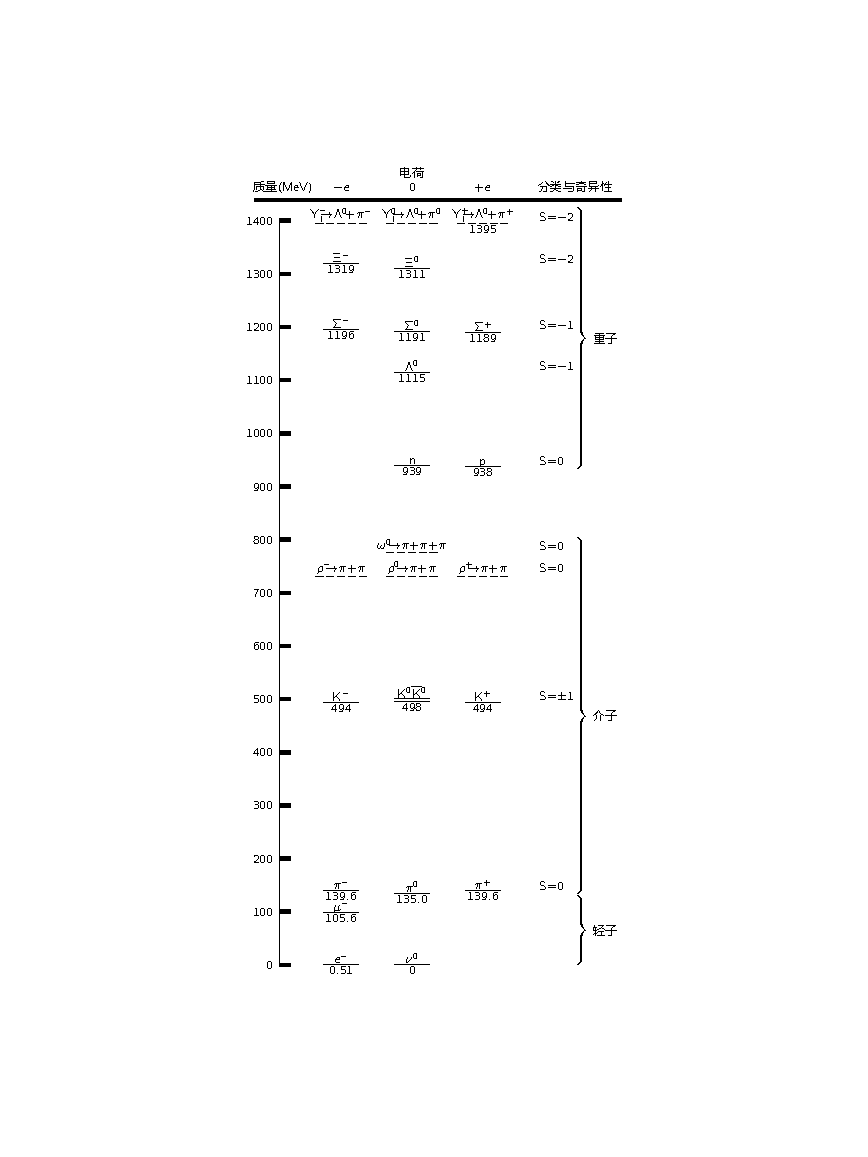
\includegraphics[width=0.65\textwidth]{Chapter2/基本粒子}
    \caption{基本粒子}
    \label{figure:基本粒子}
\end{figure}

图2.1中实线标出的是粒子,虚线标明的是“共振态”。图中略去了几个粒子,包括重要的零质量、零电荷的粒子,即光子与引力子;它们并不属于重子-介子-轻子分类图。此外,还有某些较新的共振态($K^*$,$\phi$,$\eta$)也不包括在这里。介子的反粒子也列在表格内,但轻子与重子的反粒子就需要另列一张表了,它看起来正好是前面那表格对零电荷栏的反演。虽然除去电子、中微子、光子、引力子和质子外,所有的粒子都是不稳定的,但是在这里只列出了共振态的衰变产物。奇异数并不适用于轻子,因为它们与核之间并没有强作用。

所有与中子、质子放在一起的粒子统称为\uwave{重子}。共存在着以下几种:$\lambda$介子,质量为 1154MeV 。另外三个:($ +\Sigma $)介子,($ -\Sigma $)介子,$ \Sigma $介子,质量是相近的。这里还有成群或者说成\uwave{多重态}的粒子,带有差不多相同的质量,相差不到百分之一或二。在多重态内的每个粒子都有同样的奇异数。第一个多重态是质子-中子二重态,以后是单重态($\lambda$介子),再以后是 $ \Sigma $三重态,最后是$ \Xi $二重态。最近,在1961年,又发现少数几个粒子,但它们都是粒子吗?它们的寿命是如此短暂,当刚形成时,几乎就立刻蜕变了,所以我们不知道,它们究竟应被认为是新的粒子,还是在它们蜕变成$\lambda$介子及$\pi$介子时,后二者之间某种确定能量的“共振”作用呢?

除去重子外,其它包括在核内相互作用中的粒子称为介子。首先是$\pi$介子,有三种形态:正、负及中性;它们组成了另一多重态。我们还发现一些新的称为K介子的粒子,它们作为$ K^{+} $及$ { K }^{ 0 } $而出现。其次,每个粒子都有反粒子,除非一个粒子是它自己的反粒子。例如$\pi^{-} $和$\pi^{+} $是一对反粒子,但是$\pi^0 $是它自己的反粒子;$K^- $及$ K^+ $是反粒子对,$ { K }^{ 0 } $及$ \bar {{ K }^{ 0 } }  $也是反粒子对。附带说一下,在 1961 年我们又发现了一些介子或可能的介子。它们几乎即刻就蜕变了,有一个称为$\omega$的东西带有 780MeV 的质量,分解为三个 $\pi$ 介子,有一个还不怎么确定的东西分解为两个$\pi$介子。那些被称为介子与重子的粒子与介子的反粒子放在同一张表格里,但重子的反粒子必须放到另一张通过零电荷栏“反射”而来的表格里去。

门捷列夫周期表示是完美的,除去有一些稀土元素挂在外面。同样,这里也有一些粒子挂在表外,它们在核内的相互作用不强,跟核相互作用根本无关,跟核之间也没有强相互作用。(我们所指的是那种强的核能相互作用。)它们被称为轻子,主要有如下几种:电子,其质量很小,只有 0.510MeV;然后是$\mu$介子,质量约为电子的 206 倍。根据所有的实验,我们今天所能说的是,电子与$\mu$介子之间的差别仅仅是质量不同而已,除了$\mu$介子比电子重外,其他二者都完全一样。为什么一个比另一个重?$\mu$介子有什么用?我们不知道;此外,有一种轻子是中性的,叫做中微子,具有零质量,事实上,现在知道有两类中微子,一类与电子有关,另一类与$\mu$介子有关。

最后,还有两种与核内其他粒子间没有强作用的粒子:一个是光子,另一个(或许)是具有零质量的引力子——假如引力场也有量子力学的类比的话(引力的量子化理论还没有建立)。

什么是“零质量”?这里所标明的质量是粒子\uwave{在静止时}的质量。事实上,一个粒子具有零质量在某种程度上就意味着它不可能\uwave{静止}。光子永远不会静止的,它一直以每秒 186,000 英里(300,000 公里)的速度运动。当我们在适当的时候学习了相对论的内容后,对于质量就会理解得更多一些。

这样,我们就面对着一大群粒子,它们看来都是物质的基本组成部分。幸运的是,这些粒子彼此之间的相互作用并不\uwave{全}都是不同的。事实上,粒子之间的相互作用看来可以分为四类,按强度降低的顺序排列时,它们就是:核力、电相互作用、$\beta$衰变作用以及引力。光子与所有带电粒子会发生耦合,作用的强度用某个数(1/137)来量度。这种耦合的详细定律已经知道,那就是量子电动力学。引力和所有的能量发生耦合,但它的耦合是非常弱的,远远小于电的作用,这条定律也已经知道了。然后,还存在着所谓的弱衰变——$\beta$衰变,它使中子蜕变为质子、电子及中微子,其过程是比较缓慢的,这种作用的定律只是部分地知道。还有所谓的强相互作用,介子-重子相互作用,其强度为1,它的规律完全不知道,虽然已经知道几条法则,譬如重子的数目在任何反应中都不改变。

这些就是当代物理学惊人的状况。总结一下,我们可以这样说,在核外,看来一切都知道了;在核内,量子力学是正确的,还没有发现量子力学原理失效的情况。可以说:容纳我们所有知识的舞台是相对论空-时;也许引力也包括在空-时之中。我们不知道,宇宙是怎样开始的,我们从来没有做过实验来精确地检查在某个微小距离下的空-时观念,所以只知道在哪个距离以上我们的空-时观念行得通。我们还应当补充说:这个伟大的象棋赛的规则就是量子力学的原理,到现在为止我们可以说,这些原则应用于新的粒子时,与应用于过去已经发现的粒子一样成功。核力的起源将我们引向新的粒子,但是遗憾的是,出现的粒子实在太多,以致使我们感到迷惑不解,虽然我们已经知道在它们之间存在着一些非常出人意表的关系,但对它们的相互关系缺乏完整的理解。看来我们正摸索着前进,逐渐趋于对亚原子粒子世界的理解。但是,我们实在不清楚,在这种摸索中我们还必须走多远。

\begin{table}[H]
    \centering
    \label{tab:基本相互作用}
    \caption{基本相互作用}
    \medskip 
    \begin{tabular}{@{}lll@{}}
        \toprule
        耦合关系      & 强度             & 定律         \\ \midrule
        光子对带电粒子   & $\sim10^{-2}$  & 已知         \\
        引力对所有其他能量 & $\sim10^{-40}$ & 已知         \\
        弱衰变       & $\sim10^{-5}$  & 部分已知       \\
        介子对重子     & $\sim1$        & 不知(部分法则已知) \\ \bottomrule
    \end{tabular}
\end{table}